\documentclass{standalone}
\usepackage{tikz}
\begin{document}
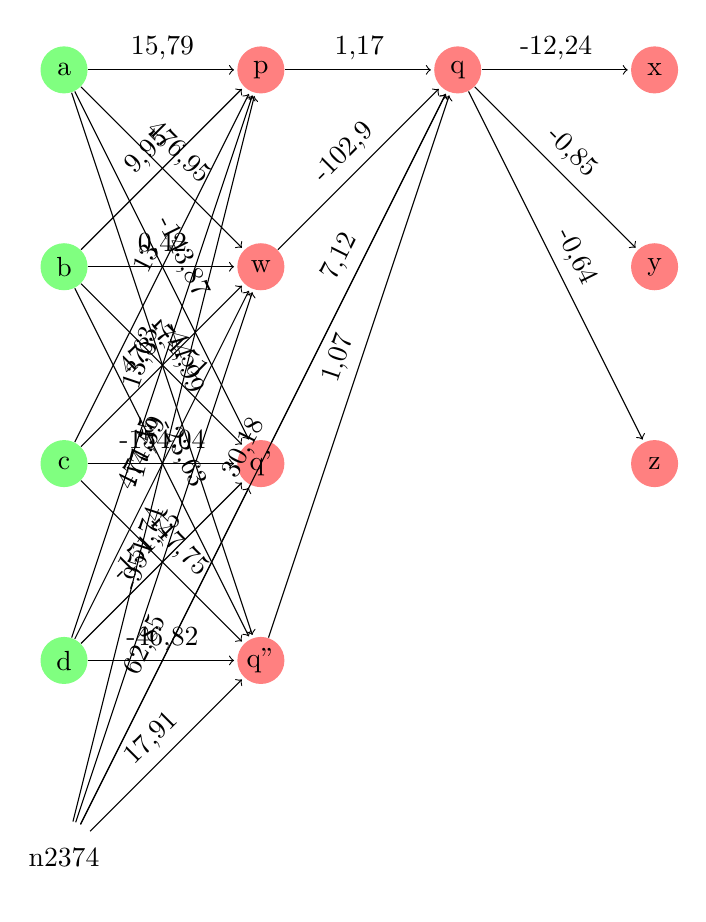
\begin{tikzpicture}[shorten >=1pt,->,draw=black!,node distance=2.5cm]
\tikzstyle{neuron}=[circle,fill=black!25,minimum size=17pt,inner sep=0pt]
\tikzstyle{constant}=[neuron, fill=white!50];
\tikzstyle{identity}=[neuron, fill=green!50];
\tikzstyle{sigmoid}=[neuron, fill=red!50];
\node [identity] (a) {a};
\node [identity,below of=a] (b) {b};
\node [identity,below of=b] (c) {c};
\node [identity,below of=c] (d) {d};
\node [constant,below of=d] (n2374) {n2374};
\node [sigmoid,right of=a] (p) {p};
\node [sigmoid,below of=p] (w) {w};
\node [sigmoid,below of=w] (q') {q'};
\node [sigmoid,below of=q'] (q'') {q''};
\node [sigmoid,right of=p] (q) {q};
\node [sigmoid,right of=q] (x) {x};
\node [sigmoid,below of=x] (y) {y};
\node [sigmoid,below of=y] (z) {z};
\path[every node/.style={sloped,anchor=south,auto=false}]
(b) edge node {0,42} (w)
(b) edge node {9,95} (p)
(b) edge node {-23,63} (q'')
(b) edge node {-74,51} (q')
(a) edge node {15,79} (p)
(a) edge node {-143,87} (q')
(a) edge node {476,95} (w)
(a) edge node {-44,99} (q'')
(d) edge node {474,59} (w)
(d) edge node {13,63} (p)
(d) edge node {-46,82} (q'')
(d) edge node {-151,75} (q')
(c) edge node {13} (p)
(c) edge node {-154,04} (q')
(c) edge node {473,7} (w)
(c) edge node {-47,75} (q'')
(n2374) edge node {-17,45} (p)
(n2374) edge node {-951,74} (w)
(n2374) edge node {30,18} (q)
(n2374) edge node {62,85} (q')
(n2374) edge node {17,91} (q'')
(w) edge node {-102,9} (q)
(p) edge node {1,17} (q)
(q'') edge node {1,07} (q)
(q') edge node {7,12} (q)
(q) edge node {-0,85} (y)
(q) edge node {-12,24} (x)
(q) edge node {-0,64} (z)
;\end{tikzpicture}
\end{document}